\documentclass[12pt]{article}
\usepackage[english]{babel}
\usepackage[utf8]{inputenc}
\usepackage{amsmath, amssymb, amsthm}
\usepackage{graphicx}
\usepackage{hyperref}
\usepackage[margin=.75in]{geometry}
\usepackage{xcolor}
\usepackage{tikz}

\newcommand{\id}{\text{id}}
\newcommand{\od}{\text{od}}

\setlength{\topmargin}{0pt}
\setlength{\headsep}{0pt}
\textheight = 600pt

\title{Graph Theory \\ Homework 15}
\author{Ben Kallus and Ryan Friedman}
\date{Due Wednesday, April 21}

\begin{document}
\maketitle

\medskip\noindent\textbf{9.13 (c)} Proposition: All planar bipartite graphs have a vertex of degree 3 or less.
\begin{proof}
    Let $G$ be a planar bipartite graph of order $n$ and size $m$.
    Suppose that $\delta(G) \geq 4$.
    Then, by the Handshaking Lemma, $2m \geq 4n$.
    Thus, $m \geq 2n$.
    However, by Theorem 9.2 for bipartite graphs,  $m \leq 2n - 4$.
    Thus, it must be that $\delta(G) \leq 3$.
\end{proof}

\newpage
\medskip\noindent\textbf{9.14 (a)} Proposition: If $G$ is a connected plane graph of order $n \geq 5$ and size $m$, and the length of a smallest cycle in $G$ is 5, then $m \leq \frac53\left(n - 2\right)$.
\begin{proof}
    Let $G$ be a connected plane graph of order $n \geq 5$ and size $m$ such that the length of a smallest cycle in $G$ is 5.
    Let $r$ be the number of regions in $G$.
    Then, each region in $G$ has degree at least 5.
    By the Region-Shaking Lemma, $5r \leq 2m$.
    Thus, $r \leq \frac25m$.
    Therefore, by Euler's Formula, $$2 \leq n - m + \frac25m = n - \frac35m.$$
    Thus, $$m \leq \frac53(n - 2).$$
    
\end{proof}

\medskip\noindent\textbf{9.14 (b)} Proposition: The Petersen graph is nonplanar.
\begin{proof}
    The Petersen graph contains two cycles, both of length 5.
    Note that the Petersen graph has 15 edges.
    Observe that $15 \not\leq \frac53\left(10-2\right) = \frac{40}3.$
    Thus, by \textbf{(a)}, the Petersen graph is nonplanar.
\end{proof}

\medskip\noindent\textbf{9.14 (d)} Proposition: If a planar graph $G$ is of order $n < 20$, and the length of a smallest cycle in $G$ is 5, then $G$ has a vertex of degree 2 or less.
\begin{proof}
    Let $G$ be a planar graph of order $n$ such that the length of a smallest cycle in $G$ is 5, and $\delta(G) \geq 3$.
    Then, by the Handshaking Lemma, $2m \geq 3n$, so $$m \geq \frac32n.$$
    By \textbf{(a)}, $m \leq \frac53(n-2)$.
    Thus, $$\frac32n \leq \frac53(n-2).$$
    Solving for $n$, we find that $$n \geq 20.$$
    Thus, all graphs of order $n < 20$ and smallest cycle length 5 have minimum vertex degree at most 2.
\end{proof}

\newpage
\medskip\noindent\textbf{9.15} Proposition: Each planar graph of order $n \leq 11$ has minimum vertex degree 4 or less.
\begin{proof}
    Let $G$ be a planar graph of order $n$ and size $m$ such that $\delta(G) \geq 5$.
    Then, by the Handshaking Lemma, $2m \geq 5n$.
    Thus, $$m \geq \frac{5n}2.$$
    By Theorem 9.2, $m \leq 3n - 6.$
    Thus, $$\frac{5n}2\leq 3n-6.$$
    Solving for $n$, we find that $$n \geq 12.$$
    Thus, all graphs of order $n \leq 11$ have minimum vertex degree at most 4.
\end{proof}

\newpage
\medskip\noindent\textbf{10.2 (b)} Proposition: For all $n \in \mathbb N$, $\chi(Q_n) = 2$.
\begin{proof}
    Observe that $Q_1 = K_2$ is bipartite, because it contains no cycles, and thus no odd cycles.
    Suppose that $Q_{n}$ is bipartite for some $n \in \mathbb N$.
    Then, by Theorem 10.2, $Q_{n}$ has a 2-coloring.
    We construct a 2-coloring for $Q_{n+1}$ by beginning with two copies of $Q_n$, one colored with red and blue, and the other colored blue where its twin is red, and red where its twin is blue.
    We then complete our construction by adding edges between corresponding vertices.
    Because none of these edges join vertices of different colors, this construction yields a valid 2-coloring for $Q_{n+1}$.
    Thus, by Theorem 10.2, $\chi(Q_{n+1}) = 2$.
    Thus, by induction, $\chi(Q_{n+1}) = 2$ for all $n \in \mathbb N$.
\end{proof}

\medskip\noindent\textbf{10.2 (c)} Proposition: Let $n \in \mathbb N$ such that $n \geq 3$. Then, $\chi(W_n) = 3$ if and only if $n$ is even, and $\chi(W_n) = 4$ if and only if $n$ is odd.
\begin{proof}
    Let $n \geq 3$ be a natural number.
    
    Suppose that $n$ is even.
    Then, $\chi(C_n) = 2$ because $C_n$ is bipartite by Theorem 1.12.
    Consider $W_n$, the graph constructed from $C_n$ by the addition of a new vertex of degree $n$.
    Because this new vertex is adjacent to every vertex in $C_n$, it cannot share a color with any of them in a coloring of $W_n$.
    Thus, $\chi(W_n) \geq 3$.
    To create a 3-coloring for $W_n$, we begin with a 2-coloring for $C_n$, then assign the vertex of degree $n$ its own, new color.
    Thus, $\chi(W_n) = 3$.

    Now, suppose that $n$ is odd.
    Then, $\chi(C_n) = 3$ because $C_n$ is not bipartite, but a 3-coloring of $C_n$ is obtained by coloring the first ${n-1}$ vertices of $C_n$ alternating colors, then coloring the remaining vertex with a new color.
    Consider $W_n$, the graph constructed from $C_n$ by the addition of a new vertex of degree $n$.
    Because this new vertex is adjacent to every vertex in $C_n$, it cannot share a color with any of them in a coloring of $W_n$.
    Thus, $\chi(W_n) \geq 4$.
    To create a 4-coloring for $W_n$, we begin with a 3-coloring for $C_n$, then assign the vertex of degree $n$ its own, new color.
    Thus, $\chi(W_n) = 4$.

\end{proof}

\newpage
\medskip\noindent\textbf{10.4 (a)} Proposition: There exists a planar graph $G$ that contains a triangle such that $\chi(G) \neq 3$.
\begin{proof}
    Consider $K_4$.
    Any set of three vertices in $K_4$ induce a triangle in $K_4$, so $K_4$ clearly contains a triangle.
    Observe that $\chi(K_4) = 4$, because all vertices are adjacent, so none may share a color.
\end{proof}

\medskip\noindent\textbf{10.4 (b)} Proposition: There exists a a graph $G$ with a 4-coloring such that $\chi(G) \neq 3$.
\begin{proof}
    Copnsider the graph $N_4$.
    A 4-coloring of $N_4$ is obtained by coloring each of its vertices with a new color.
    However, because there are no edges in $N_4$, each vertex can be assigned the same color, so $\chi(N_4) = 1 \neq 4$.
\end{proof}

\medskip\noindent\textbf{10.4 (c)} Proposition: There exists a graph $G$ such that there is no 3-coloring of $G$ and $\chi(G) \neq 4$.
\begin{proof}
    Consider the graph $K_5$.
    Then, there is clearly no 3-coloring of $K_5$, because each pair of vertices is adjacent, so $\chi(K_5) = 5$.
    Thus, $\chi(K_5) \neq 4$.
\end{proof}

\medskip\noindent\textbf{10.4 (d)} Proposition: There exists a nonplanar graph $G$ with $\chi(G) \leq 4$.
\begin{proof}
    Observe that the Petersen graph has chromatic number less than or equal to 4:
    \begin{center}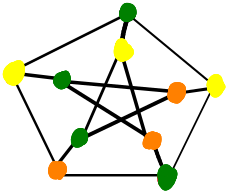
\includegraphics{fig2.png}\end{center}
    The Petersen graph is nonplanar by \textbf{9.14 (b)}.
\end{proof}

\newpage
\medskip\noindent\textbf{10.8 (a)} Proposition: There is no planar graph with chromatic number 5.
\begin{proof}
    By Theorem 10.1, a planar graph must have chromatic number less than or equal to 4.
    Thus, there is no planar graph with chromatic number 5.
\end{proof}

\medskip\noindent\textbf{10.8 (b)} Proposition: There exists a nonplanar graph with chromatic number 3.
\begin{proof}
    By \textbf{9.14 (b)}, the Petersen graph is nonplanar.
    Because the Petersen graph contains a 5-cycle, it is not bipartite by Theorem 1.12.
    Thus, its chromatic number is greater than or equal to 3.
    Consider the following figure:
    \begin{center}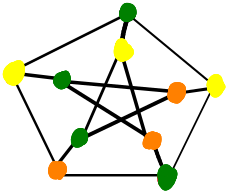
\includegraphics{fig2.png}\end{center}
    Thus, the Petersen graph's chromatic number is less than or equal to 3.
    Thus, $\chi(PG) = 3$.
\end{proof}

\medskip\noindent\textbf{10.8 (c)} Proposition: There exists a graph $G$ such that $\Delta(G) = 2\chi(G)$.
\begin{proof}
    Let $G = K_{1,4}$.
    Then, because $G$ is bipartite and nonempty, $\chi(G) = 2$ by Theorem 10.2.
    Clearly, $\Delta(G) = 4$, so $\Delta(G) = 4 = 2 \cdot 2 = 2\chi(G)$.
\end{proof}

\medskip\noindent\textbf{10.8 (d)} Proposition: There exists a graph $G$ such that $\chi(G) = 2\Delta(G)$.
\begin{proof}
        Let $G = K_2$.
        Then, $\chi(G) = 2$ because every pair of vertices in $G$ is adjacent, so each vertex needs its own color.
        Note that $\Delta(G) = 1$.
        Thus, $\chi(G) = 2 = 2 \cdot 1 = 2\Delta(G)$.
\end{proof}

\medskip\noindent\textbf{10.8 (e)} Proposition: If $G$ is a noncomplete graph of order $n$, then $\chi(G) \neq n$.
\begin{proof}
    Let $G$ be a noncomplete graph of order $n$.
    We construct a coloring for $G$ by first coloring each vertex with its own color.
    Because $G$ is noncomplete, there exists a pair of nonadjacent vertices in $G$.
    We then alter the color of one of those vertices to match the color of the other.
    Because these vertices are nonadjacent, this produces a valid $(n-1)$-coloring for $G$, so $\chi(G) \neq n$.
\end{proof}

\newpage
\medskip\noindent\textbf{10.10}

    We first construct a graph $G$ with one vertex for each course, in which two vertices are adjacent if and only if those courses share a student.
    The chromatic number of this graph is equal to the minimum number of disjoint time slots required for all students to take their exams.
    $G$ is shown below:
    \begin{center}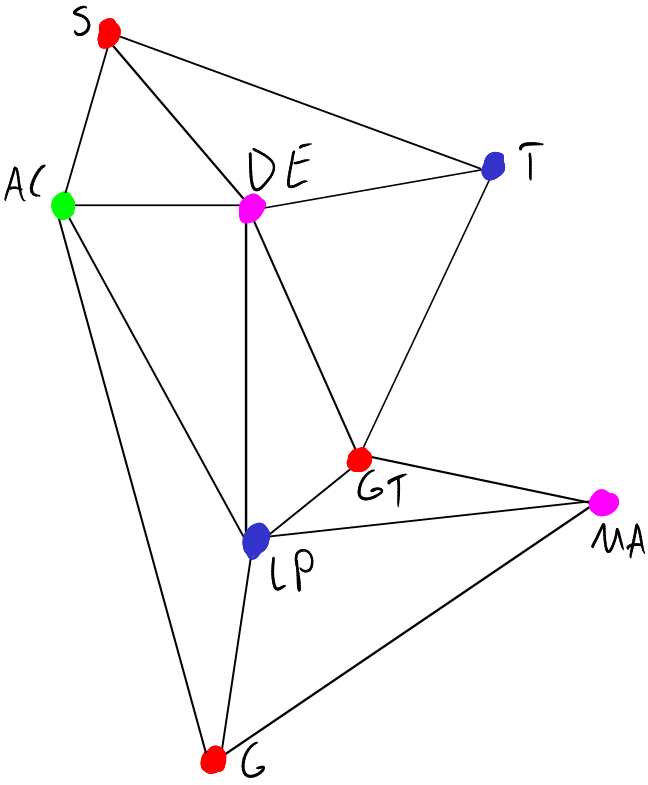
\includegraphics[scale=.5]{fig3.png}\end{center}
        Note that the subgraph of $G$ induced by $\{\text{DE}, \text{T}, \text{AC}, \text{S}, \text{GT}, \text{LP}\}$ is isomorphic to $W_5$, by \textbf{10.2 (c)}, $\chi(G) \geq 4$.
    Because we have shown $G$ with a 4-coloring, $\chi(G) = 4$.
    Thus, a minimum of four time slots are required for the students to take their exams, so the earliest they can all finish is 4:45.
\end{document}
